\documentclass[10pt,twocolumn]{article}
\usepackage[margin=0.75in]{geometry}
\usepackage{iftex}
\ifXeTeX  % local build (tectonic)
  \usepackage{fontspec}\setmainfont{texgyretermes}[Extension=.otf, UprightFont=*-regular,
    BoldFont=*-bold, ItalicFont=*-italic, BoldItalicFont=*-bolditalic]
\else     % arXiv (pdflatex)
  \usepackage{newtxtext,newtxmath}
\fi
\usepackage{amsmath,amssymb}
\usepackage{booktabs}
\usepackage{graphicx}
\usepackage{xcolor}
\usepackage[colorlinks=true,linkcolor=blue,citecolor=blue,urlcolor=blue]{hyperref}
\usepackage{caption}
\captionsetup{font=small}

\newcommand{\repourl}{\url{https://github.com/thejenilsoni/llm-cascade-audit}}

\title{\textbf{Do LLM Cascades Need Smart Stopping?\\A Real-Data Audit of Deferral Rules}}
\author{Jenil Soni\\[2pt]
\small Anybody Can AI \quad\textbar\quad \texttt{jenil@anybodycan-ai.com}}
\date{}

\begin{document}
\maketitle

\begin{abstract}
An LLM cascade sends a query to a cheap model first and escalates to larger models only when needed;
its \emph{deferral rule} decides when to stop. Increasingly sophisticated rules have been proposed,
often evaluated in simulation or against a single global confidence threshold. We audit seven rules
on real per-question log-likelihoods of 13 open models from three families (Qwen1.5 0.5B--72B,
Llama-2 7B--70B, Mistral/Mixtral) on 16{,}481 questions from MMLU, ARC-Challenge and WinoGrande,
taken from the public Open LLM Leaderboard logs. Under a protocol in which every rule is tuned on
held-out data only, we find: (i) moving from one global threshold to per-stage thresholds gains
0.8--4.3 AUCC points, more than any further, more sophisticated rule adds on top; (ii) choosing
\emph{which} models to chain (a subset cascade) is best in two of three families, degrades least with
few labels, and survives task shift, reaching 99\% of the largest model's accuracy at 74\% (Qwen) and
81\% (Mistral) of its cost; (iii) a value-of-computation lookahead rule that looked strong in our own
earlier simulation is never the best rule on real data, and its category conditioning hurts in two
of three families; (iv) in a controlled sweep, adaptive rules overtake simple model selection only
once confidence AUROC exceeds roughly 0.9, above today's real signals (0.74--0.81), at which point
matching the largest model can cost as little as 8\% of it. The practical lesson is to tune thresholds
per stage, choose the model subset, and invest in confidence quality before stopping-rule
sophistication. Code, data-fetching scripts and all results are released.
\end{abstract}

\section{Introduction}
Serving every query with the largest model is expensive, yet many queries are answered correctly by
much smaller ones. \emph{Cascades} exploit this: a query goes to the cheapest model first and is
escalated to larger models only when a deferral rule judges the current answer unreliable
\cite{frugalgpt,jitkrittum2023}. The rule is the crux of the design, and the literature has moved
from confidence thresholds \cite{frugalgpt} to learned post-hoc deferral \cite{jitkrittum2023,gupta2024},
answer-consistency signals \cite{yue2024}, provably optimal cascade routing \cite{dekoninck2025},
decision-theoretic characterisations \cite{bouchard2026} and online optimal-stopping formulations
\cite{belloni2026}; a recent survey maps the space \cite{moslem2026survey}.

Two evaluation habits make it hard to know how much this sophistication buys in practice. First, new
rules are often compared against a \emph{single global threshold} shared by all stages, a baseline
that ignores that escalation costs differ sharply between stages. Second, evidence is often simulated
or drawn from few models. We ran into both ourselves: in unpublished simulation experiments, a
value-of-computation lookahead rule we proposed (VoC-Stop, \S\ref{sec:methods}) appeared to cut cost by
17--74\% at matched accuracy against a global threshold. When we added a per-stage baseline inside the
same simulator, most of that saving disappeared, and on real data the rule was never the best.

This paper is the audit we should have run first. We use public per-question log-likelihoods for 13
open models \cite{openllmlb}, which let us evaluate any cascade offline, for free, on real correctness
and real confidence. Our contributions are:
\begin{enumerate}\itemsep1pt
\item A reproducible real-data benchmark for deferral rules: three model families, 16{,}481 questions,
  one protocol under which every rule is tuned on held-out data only (\S\ref{sec:setup}).
\item Five experiments: main comparison, confidence quality, label budget, task shift and an ablation
  (\S\ref{sec:results}), with four findings summarised in the abstract.
\item A measured account of why a simulator overstated a method's value (\S\ref{sec:sim}), and practical
  guidance for practitioners (\S\ref{sec:discussion}).
\end{enumerate}

\section{Related Work}
\paragraph{Cascades and deferral.} FrugalGPT \cite{frugalgpt} popularised LLM cascades with learned
score thresholds. Jitkrittum et al.\ \cite{jitkrittum2023} characterise the optimal deferral rule and
show when confidence-based deferral suffices and when post-hoc learned deferral helps; Gupta et
al.\ \cite{gupta2024} extend this to generative LMs using token-level uncertainty. Yue et
al.\ \cite{yue2024} use answer consistency of the weaker model as the deferral signal. Dekoninck et
al.\ \cite{dekoninck2025} unify routing and cascading and derive an optimal strategy, identifying the
quality estimator as the key factor, which our confidence sweep corroborates from a different angle.
Bouchard \cite{bouchard2026} characterises cascades with constrained optimisation over eight models and
concludes that performance is limited primarily by structural cost; our subset-cascade and
single-model results are consistent with this. Belloni et al.\ \cite{belloni2026} cast contextual
cascading as an online Pandora's-box problem. RouterBench \cite{routerbench} standardised
routing evaluation.
\paragraph{Our angle.} We do not propose a new rule. We ask how much existing rule families gain
over \emph{properly tuned} simple baselines on real logs, and when sophistication starts to pay.
The value-of-computation view we test comes from rational metareasoning \cite{russellwefald};
calibration uses isotonic regression \cite{guo2017}.

\section{Setup}\label{sec:setup}
\paragraph{Data.} The Open LLM Leaderboard (v1) \cite{openllmlb} evaluated models with the LM
Evaluation Harness \cite{lmeval} and published per-question details, including the log-likelihood of
every answer option. We use MMLU (5-shot) \cite{mmlu}, ARC-Challenge (25-shot) \cite{arc} and
WinoGrande (5-shot) \cite{winogrande} for three cascades of base models: Qwen1.5
\{0.5, 1.8, 4, 7, 14, 32, 72\}B \cite{qwen}, Llama-2 \{7, 13, 70\}B \cite{llama2} and Mistral-7B
$\to$ Mixtral-8x7B $\to$ Mixtral-8x22B \cite{mistral,mixtral}. Questions are aligned across models
by a hash of the question text, giving 16{,}481 questions answered by every model. Accuracies match the
published leaderboard values (e.g.\ Llama-2-70B MMLU 69\%, Mixtral-8x7B 70\%).
\paragraph{Confidence and categories.} A model's confidence is the maximum softmax probability over
the option log-likelihoods. Its AUROC for predicting the model's own correctness ranges from 0.62
(Qwen1.5-0.5B) to 0.83 (Mixtral-8x22B). Categories are the four MMLU super-categories plus ARC and
WinoGrande.
\paragraph{Cost.} Per-query cost is proportional to active parameters (prompts are identical across
models); Mixtral uses active parameters (12.9B, 39B). A cascade pays for every model it runs.
\paragraph{Protocol.} Each run splits questions 50/50 into train and test. Per-stage isotonic
calibration and every rule's parameters are fitted on train only; all numbers are on test, averaged
over 5 random splits (3 for E2 and E3). Rules trade accuracy for cost through an exchange rate
$\lambda$: at each of 30 log-spaced $\lambda$ values a rule is tuned to maximise
$\text{accuracy} - \text{cost}/\lambda$ on train, tracing an accuracy--cost frontier on test.
\paragraph{Metrics.} \textbf{AUCC} is the area under the (monotone envelope of the) test accuracy--cost
frontier over the cost range from the cheapest model to running every model, normalised to $[0,1]$
on the cost axis. \textbf{Cost@99} is the cost needed to reach 99\% of the largest model's accuracy,
as a percentage of calling the largest model alone.

\section{Rules Compared}\label{sec:methods}
Stages $s=1,\dots,M$ are ordered by cost; $\hat p_s$ is the calibrated confidence at stage $s$ and $z$
the category.
\begin{itemize}\itemsep1pt
\item \textbf{Global threshold}: stop at the first stage with $\hat p_s \ge \tau$, one $\tau$ for all stages.
\item \textbf{Per-stage threshold}: one $\tau_s$ per stage (as in FrugalGPT), tuned by coordinate ascent
  initialised at the best global threshold, so it is never worse than the global rule on train.
\item \textbf{Per-stage + category threshold}: separate per-stage thresholds for each category.
\item \textbf{VoC-Stop} (our earlier proposal): continue iff
  $\max_{t>s}\,[\hat g_{s\to t}(\hat p_s, z) - (C_t - C_s)/\lambda] > \hat p_s$, where
  $\hat g_{s\to t}$ is an isotonic estimate of stage-$t$ accuracy given the current confidence within
  category $z$ and $C_s$ is cumulative cost: a value-of-computation lookahead rule.
\item \textbf{Learned deferral (GBM)}: gradient-boosted estimates of $P(\text{stage }t\text{ correct}
  \mid \hat p_1,\dots,\hat p_s, z)$ plugged into the same lookahead decision, a post-hoc deferral rule
  in the spirit of \cite{jitkrittum2023,gupta2024}.
\item \textbf{Subset cascade}: for each $\lambda$, choose on train which models to run (any cost-ordered
  subset of at most three) and their per-stage thresholds; only models in the subset are paid for.
  This is a simple form of the model selection that cascade routing \cite{dekoninck2025} performs;
  we do not reimplement their full method.
\item \textbf{Single models}: call one model only (no cascade). \textbf{Oracle}: stop, per question, at
  the stage that is best in hindsight (upper bound).
\end{itemize}

\section{Results}\label{sec:results}
\begin{table*}[t]\centering\small
\caption{E1: main comparison on real data (16{,}481 questions; mean $\pm$ s.d.\ over 5 random splits; every method tuned on the training half only). AUCC: area under the accuracy--cost curve (higher is better). Cost@99: cost to reach 99\% of the largest model's accuracy, as \% of calling that model alone (-- = not reached in every split). Best non-oracle AUCC in bold.}\label{tab:main}
\begin{tabular}{lrrrrrr}\toprule
 & \multicolumn{2}{c}{Qwen1.5 (7 models)} & \multicolumn{2}{c}{Llama-2 (3)} & \multicolumn{2}{c}{Mistral (3)}\\
\cmidrule(lr){2-3}\cmidrule(lr){4-5}\cmidrule(lr){6-7}
Method & AUCC & Cost@99 & AUCC & Cost@99 & AUCC & Cost@99\\\midrule
Global threshold & 0.668\,{\scriptsize$\pm$0.008} & 112\% & 0.584\,{\scriptsize$\pm$0.009} & 111\% & 0.726\,{\scriptsize$\pm$0.004} & 98\%\\
Per-stage threshold & 0.711\,{\scriptsize$\pm$0.002} & 96\% & 0.603\,{\scriptsize$\pm$0.006} & 109\% & 0.734\,{\scriptsize$\pm$0.002} & 94\%\\
Per-stage + category thr. & 0.713\,{\scriptsize$\pm$0.002} & 101\% & 0.616\,{\scriptsize$\pm$0.003} & 107\% & 0.737\,{\scriptsize$\pm$0.002} & 93\%\\
VoC-Stop & 0.696\,{\scriptsize$\pm$0.002} & -- & 0.615\,{\scriptsize$\pm$0.003} & -- & 0.731\,{\scriptsize$\pm$0.002} & 122\%\\
Learned deferral (GBM) & 0.708\,{\scriptsize$\pm$0.002} & -- & \textbf{0.619\,{\scriptsize$\pm$0.002}} & -- & 0.734\,{\scriptsize$\pm$0.003} & --\\
Subset cascade ($\le$3) & \textbf{0.724\,{\scriptsize$\pm$0.002}} & 74\% & 0.608\,{\scriptsize$\pm$0.011} & 100\% & \textbf{0.740\,{\scriptsize$\pm$0.003}} & 81\%\\
Single models (no cascade) & 0.721\,{\scriptsize$\pm$0.002} & 100\% & 0.593\,{\scriptsize$\pm$0.003} & 100\% & 0.725\,{\scriptsize$\pm$0.003} & 100\%\\
\midrule
Oracle (upper bound) & 0.899\,{\scriptsize$\pm$0.002} & 4\% & 0.778\,{\scriptsize$\pm$0.003} & 30\% & 0.843\,{\scriptsize$\pm$0.003} & 23\%\\
\bottomrule\end{tabular}
\end{table*}


\paragraph{E1: main comparison (Table~\ref{tab:main}, Fig.~\ref{fig:frontier}).}
Three patterns hold across families. \emph{The global threshold is the weakest cascade rule
everywhere}; per-stage thresholds improve AUCC by 0.043 (Qwen), 0.019 (Llama-2) and 0.008 (Mistral),
more than the best further gain any other rule achieves over per-stage thresholds (0.013, 0.016 and
0.006 respectively). \emph{Model selection matters}: the subset cascade is best on Qwen and Mistral,
typically chaining two large models (e.g.\ 32B$\to$72B), and reaches 99\% of the largest model's
accuracy at 74\% and 81\% of its cost. On Llama-2, where the 70B model is far more accurate than the
13B (70\% vs 57\%), no rule saves cost at the 99\% target, and learned deferral has the best AUCC.
\emph{VoC-Stop is never the best rule}: it trails per-stage thresholds on Qwen and Mistral and trails
learned deferral on Llama-2. The oracle's large margin (4--30\% Cost@99) shows ample headroom, which
the next experiment attributes to confidence quality.

\begin{figure*}[t]\centering
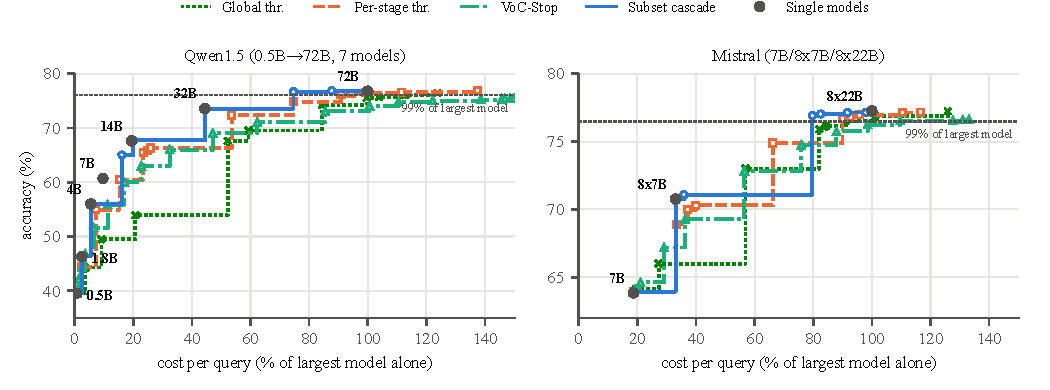
\includegraphics[width=0.92\textwidth]{figures/fig_frontier.pdf}
\caption{Accuracy--cost frontiers on real data (one test split). Dots are single models. The subset
cascade (blue) dominates the full-ladder rules on Qwen1.5 and Mistral; the global threshold (green,
dotted) is weakest.}\label{fig:frontier}
\end{figure*}

\begin{figure*}[t]\centering
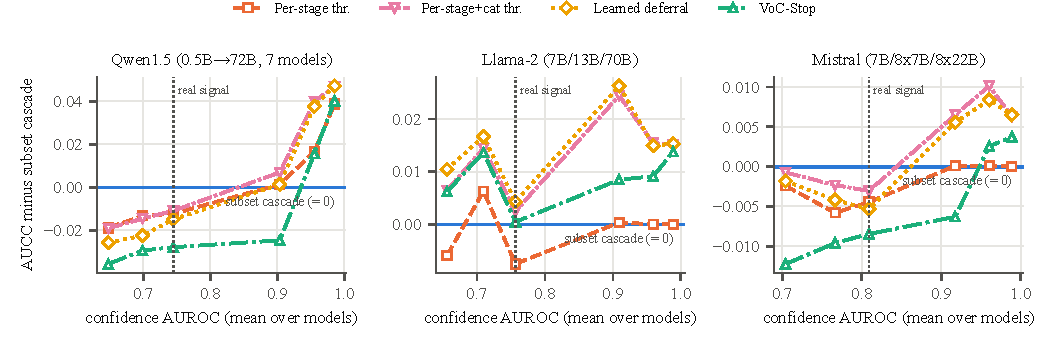
\includegraphics[width=0.95\textwidth]{figures/fig_confidence.pdf}
\caption{E2: AUCC of each rule minus the subset cascade as confidence quality varies. Points left of
the dashed line are noised versions of the real signal; points to the right are label-sharpened
(not deployable). On Qwen1.5 and Mistral, adaptive rules overtake simple model selection only
around AUROC 0.9.}\label{fig:conf}
\end{figure*}

\begin{table*}[t]\centering\small
\caption{E2: AUCC as confidence quality varies (3 splits). Sharpened signals use the label and are \emph{not} deployable; they show what a better confidence estimator would buy. Best non-oracle in bold.}
\label{tab:conf}
\begin{tabular}{llrrrrrr}\toprule
 & Signal & AUROC & Per-stage & PS+cat & GBM & VoC-Stop & Subset\\\midrule
Qwen & noised ($\sigma{=}2$) & 0.65 & 0.704 & 0.704 & 0.697 & 0.687 & \textbf{0.723}\\
 & noised ($\sigma{=}1$) & 0.70 & 0.710 & 0.709 & 0.701 & 0.694 & \textbf{0.723}\\
 & \textit{real (max-prob)} & 0.74 & 0.712 & 0.713 & 0.709 & 0.696 & \textbf{0.724}\\
 & sharpened ($\beta{=}0.5$) & 0.90 & 0.771 & \textbf{0.777} & 0.771 & 0.745 & 0.770\\
 & sharpened ($\beta{=}1$) & 0.96 & 0.821 & \textbf{0.845} & 0.842 & 0.820 & 0.804\\
 & sharpened ($\beta{=}2$) & 0.99 & 0.875 & 0.883 & \textbf{0.884} & 0.877 & 0.836\\
\midrule
Llama-2 & noised ($\sigma{=}2$) & 0.66 & 0.592 & 0.604 & \textbf{0.608} & 0.604 & 0.597\\
 & noised ($\sigma{=}1$) & 0.71 & 0.602 & 0.610 & \textbf{0.612} & 0.609 & 0.596\\
 & \textit{real (max-prob)} & 0.76 & 0.606 & 0.616 & \textbf{0.618} & 0.614 & 0.614\\
 & sharpened ($\beta{=}0.5$) & 0.91 & 0.671 & 0.695 & \textbf{0.697} & 0.679 & 0.671\\
 & sharpened ($\beta{=}1$) & 0.96 & 0.720 & \textbf{0.736} & 0.735 & 0.729 & 0.720\\
 & sharpened ($\beta{=}2$) & 0.99 & 0.740 & 0.755 & \textbf{0.755} & 0.753 & 0.740\\
\midrule
Mistral & noised ($\sigma{=}2$) & 0.70 & 0.723 & 0.725 & 0.724 & 0.713 & \textbf{0.725}\\
 & noised ($\sigma{=}1$) & 0.77 & 0.728 & 0.731 & 0.729 & 0.724 & \textbf{0.733}\\
 & \textit{real (max-prob)} & 0.81 & 0.735 & 0.736 & 0.734 & 0.731 & \textbf{0.740}\\
 & sharpened ($\beta{=}0.5$) & 0.92 & 0.776 & \textbf{0.782} & 0.781 & 0.769 & 0.776\\
 & sharpened ($\beta{=}1$) & 0.96 & 0.804 & \textbf{0.814} & 0.812 & 0.806 & 0.804\\
 & sharpened ($\beta{=}2$) & 0.99 & 0.822 & 0.829 & \textbf{0.829} & 0.826 & 0.822\\
\bottomrule\end{tabular}
\end{table*}


\paragraph{E2: confidence quality decides whether sophistication pays (Fig.~\ref{fig:conf},
Table~\ref{tab:conf}).} We perturb the real confidence in logit space: adding Gaussian noise degrades
it; adding $\beta(2y-1)$, where $y$ is correctness, sharpens it. Sharpening uses the label and is
not deployable; it answers ``what would a better confidence estimator buy?''. On Qwen and Mistral the
subset cascade wins at and below real signal quality (AUROC 0.74 and 0.81), and adaptive rules
(per-stage + category, learned deferral) overtake it only around AUROC 0.90--0.92. With better
confidence the cost of matching the largest model collapses: on Qwen, Cost@99 falls from 73\% with
real confidence to 8\% at AUROC 0.96. On Llama-2 the adaptive rules lead at every quality level.
Three alternative real signals from the same logs (top-two margin, normalised entropy, agreement with
the previous model) all had AUROC within 0.04 of max-probability and did not change the ranking.

\begin{figure*}[t]\centering
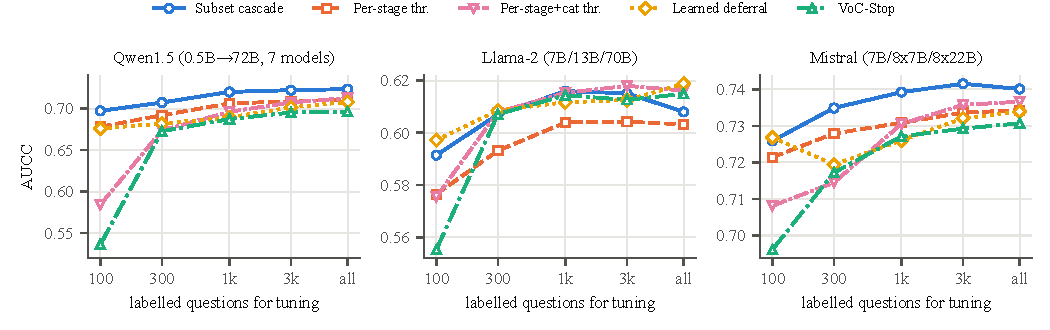
\includegraphics[width=0.95\textwidth]{figures/fig_labels.pdf}
\caption{E3: AUCC vs.\ number of labelled questions used for tuning (3 splits). The subset cascade is
near its full-data value with 100 labels; VoC-Stop and category thresholds need 300--3{,}000.}
\label{fig:labels}
\end{figure*}

\paragraph{E3: label budget (Fig.~\ref{fig:labels}).} Deployments often have few labelled examples.
With 100 labels the subset cascade stays within 0.03 AUCC of its full-data value in every family,
whereas VoC-Stop loses 0.16 (Qwen), 0.06 (Llama-2) and 0.03 (Mistral) and category thresholds lose up
to 0.13. Rules that condition on more context need more data, and on Qwen and Mistral they do not
recover their deficit even with all 8{,}240 training questions.

\paragraph{E4: task shift (Table~\ref{tab:shift}).} Tuning on MMLU and testing on ARC and WinoGrande,
the subset cascade remains best on Qwen (Cost@99 62\%) and Mistral (64\%). On Llama-2 all rules are
within 0.03 AUCC; VoC-Stop is marginally best and the subset cascade falls back to the single
largest model.
\begin{table*}[t]\centering\small
\caption{E4: task shift. Rules tuned on MMLU, evaluated on ARC-Challenge + WinoGrande (category information removed; 5 training subsamples).}\label{tab:shift}
\begin{tabular}{lrrrrrr}\toprule
 & \multicolumn{2}{c}{Qwen1.5 (7 models)} & \multicolumn{2}{c}{Llama-2 (3)} & \multicolumn{2}{c}{Mistral (3)}\\
\cmidrule(lr){2-3}\cmidrule(lr){4-5}\cmidrule(lr){6-7}
Method & AUCC & Cost@99 & AUCC & Cost@99 & AUCC & Cost@99\\\midrule
Global threshold & 0.634 & -- & 0.693 & 97\% & 0.740 & 83\%\\
Per-stage threshold & 0.657 & -- & 0.696 & 87\% & 0.745 & 73\%\\
Per-stage + category thr. & 0.657 & -- & 0.696 & 87\% & 0.745 & 73\%\\
VoC-Stop & 0.659 & -- & \textbf{0.698} & 91\% & 0.745 & 81\%\\
Learned deferral (GBM) & 0.671 & -- & 0.697 & 93\% & 0.743 & 90\%\\
Subset cascade ($\le$3) & \textbf{0.695} & 62\% & 0.673 & 100\% & \textbf{0.746} & 64\%\\
Single models (no cascade) & 0.695 & 100\% & 0.673 & 100\% & 0.738 & 100\%\\
\midrule
Oracle (upper bound) & 0.835 & 3\% & 0.790 & 21\% & 0.820 & 22\%\\
\bottomrule\end{tabular}
\end{table*}


\paragraph{E5: which ingredients matter (Table~\ref{tab:ablation}).} Calibrating the confidence
changes little (at most +0.006 AUCC). Per-stage thresholds are the largest single step in every
family. For VoC-Stop, removing category conditioning \emph{improves} AUCC on Qwen (0.696$\to$0.713)
and Mistral (0.731$\to$0.736) and costs 0.003 on Llama-2, contradicting the premise that
instance-conditional value is the source of its gains. Lookahead does matter on the long, heterogeneous
Qwen ladder: the one-step (myopic) variant drops to 0.654, while on the three-model cascades the two
are within 0.003.
\begin{table*}[t]\centering\small
\caption{E5: ablation, adding one ingredient at a time (5 splits).}\label{tab:ablation}
\begin{tabular}{lrrrrrr}\toprule
 & \multicolumn{2}{c}{Qwen1.5 (7 models)} & \multicolumn{2}{c}{Llama-2 (3)} & \multicolumn{2}{c}{Mistral (3)}\\
\cmidrule(lr){2-3}\cmidrule(lr){4-5}\cmidrule(lr){6-7}
Method & AUCC & Cost@99 & AUCC & Cost@99 & AUCC & Cost@99\\\midrule
raw confidence, global thr. & 0.662 & 164\% & 0.584 & 107\% & 0.726 & 98\%\\
Global threshold & 0.668 & 112\% & 0.584 & 111\% & 0.726 & 98\%\\
Per-stage threshold & 0.711 & 96\% & 0.603 & 109\% & 0.734 & 94\%\\
VoC, one-step (myopic) & 0.654 & -- & 0.614 & -- & 0.734 & --\\
VoC, lookahead, no category & \textbf{0.713} & 97\% & 0.612 & 108\% & 0.736 & 96\%\\
VoC-Stop & 0.696 & -- & 0.615 & -- & 0.731 & 122\%\\
Per-stage + category thr. & 0.713 & 101\% & \textbf{0.616} & 107\% & \textbf{0.737} & 93\%\\
\bottomrule\end{tabular}
\end{table*}


\section{Why the Simulation Misled}\label{sec:sim}
Our earlier simulator drew correctness from an item-response model with RouterBench-style costs and
hand-set categories whose value of escalation differed strongly. Three measured differences explain
most of the gap. (1)~\textbf{Baseline}: inside the simulator itself, replacing the global threshold
by per-stage thresholds cut VoC-Stop's saving at the GPT-3.5 operating point from 71\% to 25\%.
(2)~\textbf{Category structure}: the simulator built in categories that reward conditioning; in real
data category conditioning adds at most 0.013 AUCC to thresholds and hurts VoC-Stop in two families.
(3)~\textbf{Cost structure}: in the simulator the models before the largest cost 36\% of it in total;
in real Qwen1.5 they cost 82\%, so a full-ladder cascade pays much more before escalating, which is
why model selection matters. Cross-model correctness correlation was \emph{not} the culprit (0.14 in
simulation vs.\ 0.19--0.45 in real data). The lesson generalises: evaluate deferral rules on real logs,
and always include per-stage thresholds and single models as baselines.

\section{Discussion and Guidance}\label{sec:discussion}
For practitioners building a cascade with confidence signals like those studied here: (1)~never tune a
single global threshold; tune one per stage; (2)~search over which models to include, since two
well-chosen models often beat a full ladder; (3)~compare against simply calling a single model, since
on some families (here Llama-2 at high accuracy targets) no cascade saves cost; (4)~spend effort on
confidence quality, where the headroom is (Table~\ref{tab:conf}), before adopting context-conditioned
or lookahead rules, which are data-hungry and pay off mainly when confidence is strong.

\section{Limitations}
Models are 2023--24 open base models scored by option log-likelihood on multiple-choice tasks; modern
instruction-tuned and API models, generative tasks and verbalised confidence may behave differently,
and API models often expose no log-probabilities. Cost is modelled as active parameters, ignoring
prompt length, hardware and provider pricing. Sharpened confidence in E2 is constructed from labels
and only bounds what a better estimator could achieve. Subset search is limited to three models, we
do not reimplement the full cascade-routing method \cite{dekoninck2025}, and results average 3--5
random splits.

\section{Conclusion}
On real logs from 13 models, the sophistication of the stopping rule matters far less than three
simpler choices: tuning thresholds per stage, choosing which models to chain, and the quality of the
confidence signal. We hope the released benchmark makes it easy to hold new deferral rules to this
standard.

\paragraph{Reproducibility.} All code, the data-fetching script and every result file are at
\repourl. A single script re-runs all experiments in about 40 minutes on a desktop PC, without API keys or GPUs.

\paragraph{Use of AI tools.} AI-based coding and writing assistants were used during development of
the code and preparation of the manuscript. The author designed the study, reviewed all code and
results, and takes full responsibility for the content.

\small
\bibliographystyle{plain}
\begin{thebibliography}{99}
\bibitem{frugalgpt} L.~Chen, M.~Zaharia, J.~Zou. FrugalGPT: How to use large language models while reducing cost and improving performance. \emph{arXiv:2305.05176}, 2023.
\bibitem{jitkrittum2023} W.~Jitkrittum, N.~Gupta, A.~K.~Menon, H.~Narasimhan, A.~S.~Rawat, S.~Kumar. When does confidence-based cascade deferral suffice? In \emph{NeurIPS}, 2023.
\bibitem{gupta2024} N.~Gupta, H.~Narasimhan, W.~Jitkrittum, A.~S.~Rawat, A.~K.~Menon, S.~Kumar. Language model cascades: Token-level uncertainty and beyond. In \emph{ICLR}, 2024.
\bibitem{yue2024} M.~Yue, J.~Zhao, M.~Zhang, L.~Du, Z.~Yao. Large language model cascades with mixture of thoughts representations for cost-efficient reasoning. In \emph{ICLR}, 2024.
\bibitem{dekoninck2025} J.~Dekoninck, M.~Baader, M.~Vechev. A unified approach to routing and cascading for LLMs. In \emph{ICML}, 2025.
\bibitem{bouchard2026} D.~Bouchard. Is escalation worth it? A decision-theoretic characterization of LLM cascades. \emph{arXiv:2605.06350}, 2026.
\bibitem{belloni2026} A.~Belloni, Y.~Chen, Y.~Wei. Online Pandora's box for contextual LLM cascading. \emph{arXiv:2606.07392}, 2026.
\bibitem{moslem2026survey} Y.~Moslem, J.~D.~Kelleher. Dynamic model routing and cascading for efficient LLM inference: A survey. \emph{Transactions on Machine Learning Research}, 2026. arXiv:2603.04445.
\bibitem{routerbench} Q.~J.~Hu, J.~Bieker, X.~Li, N.~Jiang, B.~Keigwin, G.~Ranganath, K.~Keutzer, S.~K.~Upadhyay. RouterBench: A benchmark for multi-LLM routing system. \emph{arXiv:2403.12031}, 2024.
\bibitem{russellwefald} S.~Russell, E.~Wefald. Principles of metareasoning. \emph{Artificial Intelligence}, 49(1--3):361--395, 1991.
\bibitem{guo2017} C.~Guo, G.~Pleiss, Y.~Sun, K.~Q.~Weinberger. On calibration of modern neural networks. In \emph{ICML}, 2017.
\bibitem{openllmlb} E.~Beeching, C.~Fourrier, N.~Habib, S.~Han, N.~Lambert, N.~Rajani, O.~Sanseviero, L.~Tunstall, T.~Wolf. Open LLM Leaderboard (2023--2024). Hugging Face, 2023.
\bibitem{lmeval} L.~Gao et al. A framework for few-shot language model evaluation. Zenodo, 2023.
\bibitem{mmlu} D.~Hendrycks, C.~Burns, S.~Basart, A.~Zou, M.~Mazeika, D.~Song, J.~Steinhardt. Measuring massive multitask language understanding. In \emph{ICLR}, 2021.
\bibitem{arc} P.~Clark, I.~Cowhey, O.~Etzioni, T.~Khot, A.~Sabharwal, C.~Schoenick, O.~Tafjord. Think you have solved question answering? Try ARC, the AI2 reasoning challenge. \emph{arXiv:1803.05457}, 2018.
\bibitem{winogrande} K.~Sakaguchi, R.~Le~Bras, C.~Bhagavatula, Y.~Choi. WinoGrande: An adversarial Winograd schema challenge at scale. In \emph{AAAI}, 2020.
\bibitem{qwen} J.~Bai et al. Qwen technical report. \emph{arXiv:2309.16609}, 2023.
\bibitem{llama2} H.~Touvron et al. Llama 2: Open foundation and fine-tuned chat models. \emph{arXiv:2307.09288}, 2023.
\bibitem{mistral} A.~Q.~Jiang et al. Mistral 7B. \emph{arXiv:2310.06825}, 2023.
\bibitem{mixtral} A.~Q.~Jiang et al. Mixtral of experts. \emph{arXiv:2401.04088}, 2024.
\end{thebibliography}
\end{document}
